\section{Complete results: the Phase 6 reference-effect mechanisms and the income realism track}
\label{sec:p6}

The brutal-honest summary
You were partly right, partly tripping — and now you know which part.
1. Why you lost D5/D6 reference targets (the diagnostic you didn't have): your fitted 10-particle cloud under-disperses the conditional law, arm-asymmetrically. On D5 arm 0 the bias is −0.149. The reference distance is convex in spread, so Jensen's inequality biases it low and attenuates the contrast. Forests win there not because they learn better laws (R3 beats Causal-DRF on the law metric in D5) but because ~500 empirical atoms integrate a convex functional with less quantization bias than 10 atoms.
2. What fixed it (cwdb_dr): a doubly-robust AIPW layer over the untouched R3 law. D5 REF-ATE: 0.1115 → 0.0232, parity with Causal-DRF (0.0212). D0 floor: 0.0385 → 0.0058. Law metrics identical to R3 by construction (verified to machine precision). Price, honestly stated: variance on null/confounded conditional targets (+0.031 on D2 TCATE-ref). Gate R1 = PARTIAL.
3. Negative findings, with mechanisms: smoothing helps only D6 and destroys D7-skewness (gate FAIL); kernel-ridge weak learners lose everywhere because trees' "crudeness" is what averages the idiosyncratic score component — smooth learners memorize it. So no, RF-style averaging isn't the bottleneck; it's load-bearing.
4. cwdb_frl (functional R-learner): best-in-roster on scale contrasts and the most null-safe estimator in the project; weak where the contrast is x-independent (D5). A benchmark, not a claimant.
5. The income realism track flipped the story: under endogenous adoption + skewed outcomes + benchmark reference, Causal-DRF and DRF collapse — REF-TCATE 0.14–0.26 vs R3's 0.01–0.07, and they manufacture massive false effects even on the placebo (IC0). Your transfer functionals hold (3–10× better than forests). PTA-S wins only where functionals are pre-declared.
For Tanise/IPUMS: pitch the applied study around REF-ATE/REF-TCATE with cwdb_dr as the estimator — that's where you now have parity-to-superior results and a documented incumbent failure mode.

Sections~\ref{sec:complete} and~\ref{sec:complete55} left three problems open.
On the reference-distribution targets this project exists to serve,
\texttt{REF-ATE-K} and \texttt{REF-TCATE-K}, the recommended claimant loses to
both forest baselines on D5 by a factor of four to five. The pure-shape
transfer that motivated the whole representation is damaged by exactly the
contrast regularisation that fixes the null regime. And every synthetic regime
in the suite shares one Hermite inner shape, a standard-normal reference, and
an assignment mechanism unrelated to the economy it acts on, so none of them
resembles the applied study under discussion, in which each unit is a
state-year panel observation, the outcome is an income-like right-skewed
distribution, the reference is a named benchmark economy, and policy adoption
is endogenous.

Phase 6 tests four mechanisms, one variant each, plus the realism track. This
section reports what came out. Everything was frozen before the first decisive
seed in \texttt{research/simulation\_preregistration\_phase6.md}; every number
comes from the audited merge \texttt{results/merged\_phase6/} produced by
\texttt{research/run\_phase6.py}; and the tables and figures were generated by
\texttt{report/build\_phase6\_assets.py}, which reads and aggregates but never
fits a model. The four variants are \texttt{cwdb\_dr}, a doubly-robust
calibration layer over the untouched R3 law;
\texttt{cwdb\_smooth}, dispersion repair of the particle cloud chosen on
held-out energy score; \texttt{cwdb\_krr}, the particle booster with kernel-
ridge instead of tree weak learners; and \texttt{cwdb\_frl}, the functional
R-learner, which generalises Phase 5.5's orthogonalisation to arbitrary grid
functionals.

\subsection{Conventions, and four disclosed repairs}
\label{sub:p6-conventions}

The conventions carry over from Section~\ref{sec:complete55} with two changes.
First, the whole phase runs ten seeds, so every frozen-record incumbent pooled
into a table below is restricted to seeds 0 through 9; pooling a twenty-seed
mean against a ten-seed mean would compare two designs. Second, the
Causal-DRF and DRF columns are the original-code rerun record throughout, as
in Section~\ref{sec:complete}; the retired local driver rows that also live in
the frozen main file are excluded at load time rather than blended into the
same label.

Four implementation defects were found during the phase and repaired before
any claim was written, and they are recorded here because nothing else in the
preregistration discipline will record them. First, the initial income track
failed on all 480 cells before producing a single result: a wrong-arity
surface function, a broadcasting error in the benchmark reference vector, and
a wage-floor parameterisation that lowered bottom quantiles, which is the
opposite of what a wage floor does. The surfaces were repaired and every Track
B cell ran afterwards; no failed cell informed any comparison. Second, the
first screen's functional R-learner failed D5 catastrophically, and the
diagnostics traced it to a design defect: joint scalar shrinkage selection
coupled twenty-five zero-contrast coordinate columns with the one column
carrying D5's entire signal and chose a block-wide strength near 340. The
repair gives each column its own held-out-selected ridge strength from the
same fold runs. Third and fourth, a cell-level audit found the cross-fitted
variants had been run at three selection folds instead of the published R3
estimator's two, and at five particles instead of the roster's ten; both were
repaired and the affected cells rerun. After the repair, an identity check
confirms that \texttt{cwdb\_dr}'s underlying law equals
\texttt{cwdb\_r3\_cvridge}'s on all 120 shared Track A cells to machine
precision, which is what makes the attribution below clean: any difference
between the two methods is the calibration layer and nothing else.

\subsection{The opening diagnostic: why D5 was lost}
\label{sub:p6-diag}

Before any variant was chosen, the phase opened with a measurement, recorded
in Table~\ref{tab:p6-diag}: fit the frozen C-WDB-v1 booster, predict particle
clouds on a large test design, and compare the implied expectation of the
reference distance against quadrature truth, per arm, at five pilot seeds
outside every manifest.

The bias is negative wherever the conditional law has substantial outer
spread, and arm-asymmetric exactly where the arms' spreads differ. On D5,
whose arm outer location laws have standard deviations 0.40 and 0.15, the
fitted cloud understates the expected distance to the reference by $0.149$ on
arm 0 and essentially zero on arm 1. On D6 the bimodal outer location produces
biases near $-0.31$ on both arms. On D1 the bias is small and nearly
symmetric, which is why the reference targets looked mediocre rather than
broken there. The mechanism is under-dispersion of the fitted cloud, and its
consequence is structural: the reference distance is convex in spread, so
Jensen's inequality turns a too-tight cloud into a biased-low functional and
an arm-asymmetric tightness into an attenuated contrast. No shrinkage tuning
repairs this, because the bias lives in the plug-in step, not in the contrast
surface.

\begin{figure}[htbp]
\centering
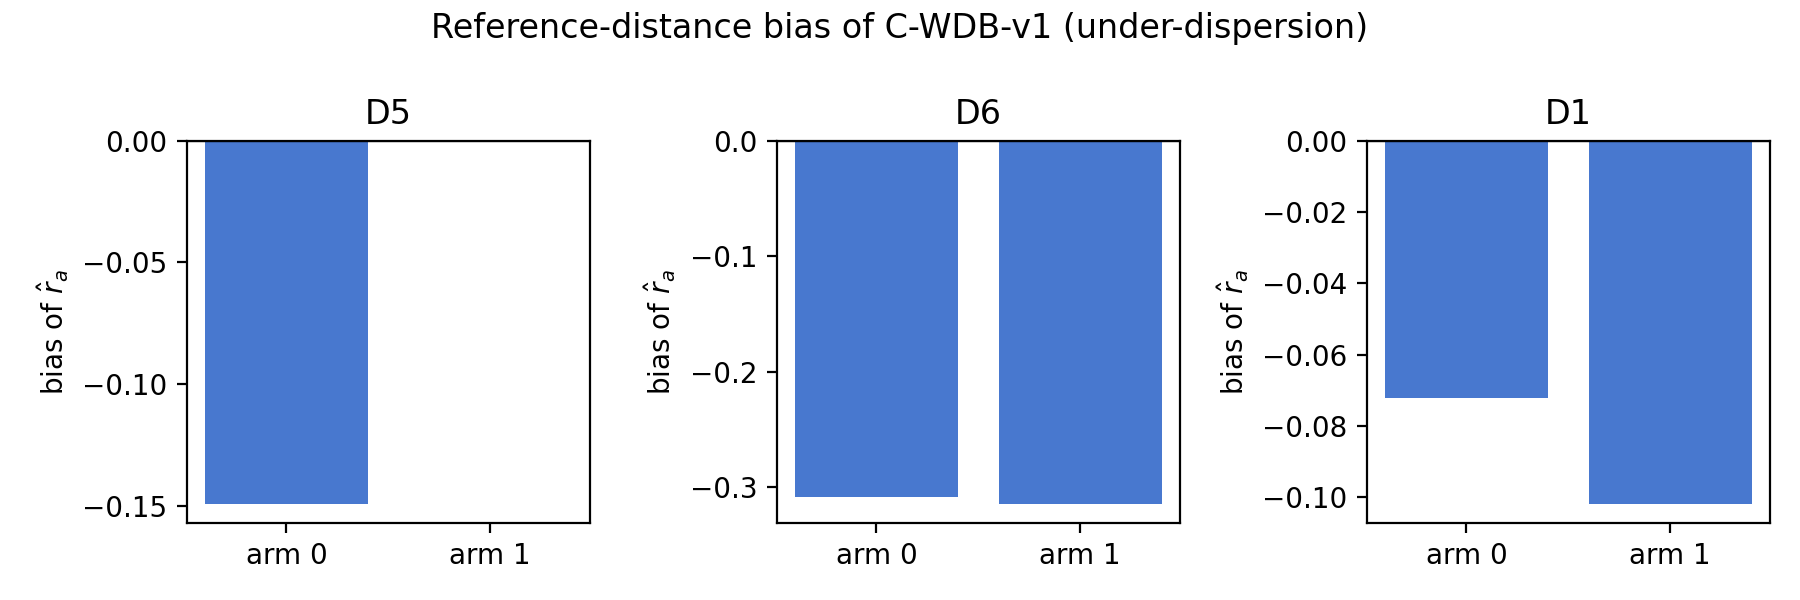
\includegraphics[width=0.95\textwidth]{figures_generated/phase6_dispersion.png}
\caption{Mean bias of the C-WDB-v1 reference-distance expectation against
quadrature truth, per arm, five pilot seeds at $n=500$. Negative means the
fitted law is too tight. The bias concentrates where the true outer spread is
largest, which is the signature of under-dispersion rather than noise.}
\label{fig:p6-dispersion}
\end{figure}

This reframes the D5 loss recorded in Section~\ref{sec:r3intournament}. It is
not that the forests estimate laws better in any global sense there; on the
primary law metric R3 beats Causal-DRF on D5 comfortably. It is that a
weighted empirical law over several hundred training outcomes integrates a
convex spread functional with little quantisation bias while ten boosted atoms
do not, and the contrast inherits the difference. Two variants below attack
exactly this, one by repairing the aggregation and one by repairing the cloud.

\subsection{Track A reference surface: the layer works where it was aimed and
pays where it was not}
\label{sub:p6-ref}

Tables~\ref{tab:p6-tracka-reference_effect_rmse}
and~\ref{tab:p6-tracka-reference_tcate_rmse} give both reference targets across
the six mechanism regimes, and Table~\ref{tab:p6-trackA-paired-ref} gives
seed-paired differences against R3 and against the incumbent.

\emph{The marginal reference effect is repaired outright.} On D5,
\texttt{cwdb\_dr} scores $0.0232$ against R3's $0.1115$, a paired difference
of $-0.0883$ at $10.9$ paired standard errors, landing at parity with
Causal-DRF ($0.0212$) and DRF ($0.0189$). On D0, whose deterministic laws give
the spread functionals their purest test, \texttt{cwdb\_dr} records $0.0058$
against R3's $0.0385$ and Causal-DRF's $0.0129$; the family-wide D0 reference
deficit disappears, because with no outer randomness the realised-arm residuals
carry exactly the plug-in bias and the correction removes it. On D8, the
strongly confounded regime, the layer does not help ($+0.0173$ paired against
R3): the propensity weights add variance where the g-computation was already
accurate, and R3 stays the best method in the roster there.

\emph{The conditional reference effect is halved, not closed.} On D5
REF-TCATE, \texttt{cwdb\_dr} improves R3 by $-0.0602$ at $7.5$ paired standard
errors but reaches only $0.0549$ against Causal-DRF's $0.0332$ and PTA-S's
$0.0289$. The reason is variance, not bias: the bin estimator averages about
125 training rows per moderator bin at $n=500$, each carrying an
inverse-propensity weight, and the paired table shows the same pattern on D2
and D8, where the truth is small or null and the g-computation was already
fine, so the layer's price is pure added noise ($+0.0306$ and $+0.0579$
paired). On D6 the layer also loses to R3, whose law is already well
calibrated there after the repairs of Section~\ref{sec:complete}. The honest
summary is that the calibration layer converts the reference targets from the
method's worst comparisons to parity on the marginal version and to a factor
two on the conditional version, at a stated variance price on nulls and under
strong confounding, and at no cost anywhere else: because the law passes
through untouched, every law-level number of R3 belongs to \texttt{cwdb\_dr}
identically.

Rule R1 of the preregistration asked for the D5 repair without significant
losses on D2 or D8, and it returns PARTIAL as written: both D5 repairs clear
their thresholds, and the D2 and D8 losses are real. Rule R2, the inherited
null-safety cap, passes everywhere precisely because the law is untouched (D0
and D2 means equal R3's own, and the D2 false-effect ratio is 1.08 against a
cap of 1.25).

\begin{figure}[htbp]
\centering
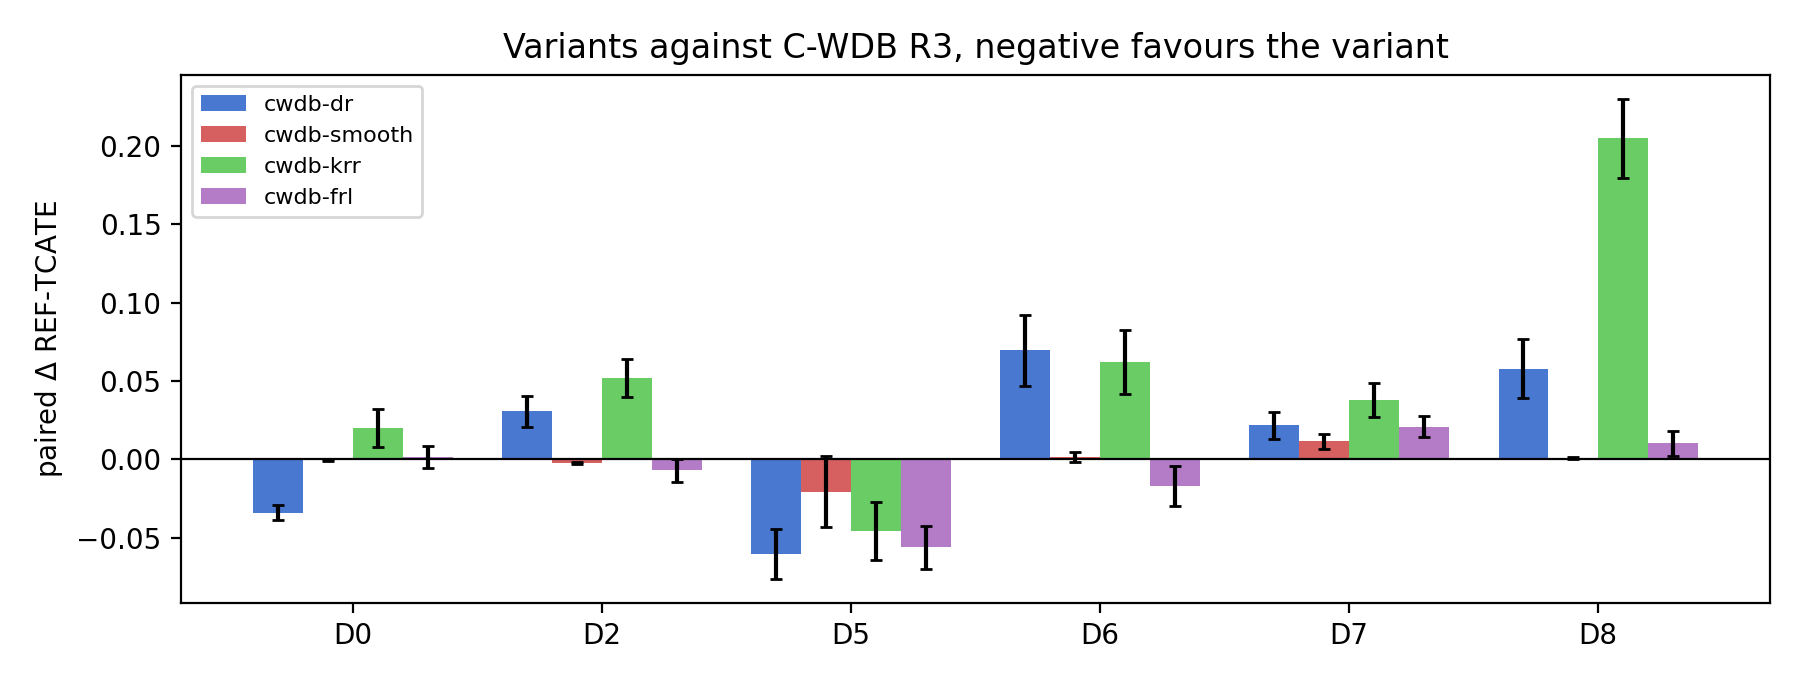
\includegraphics[width=0.98\textwidth]{figures_generated/phase6_trackA_ref_paired.png}
\caption{Seed-paired REF-TCATE differences of each variant against C-WDB R3,
worst cases visible per regime, bars at two paired standard errors. Negative
favours the variant. The calibration layer owns D5 and D0; the functional
R-learner owns the null and multimodal regimes.}
\label{fig:p6-paired}
\end{figure}

\subsection{Track A law surface: smoothing is a D6 tool, and the smooth weak
learner is a negative finding with a mechanism}
\label{sub:p6-law}

Table~\ref{tab:p6-trackA-kernel_law_error} gives the primary law metric.
Three readings, one of them uncomfortable.

\emph{The calibration layer leaves the law exactly where R3 left it}, by
construction, and the tables confirm the identity rather than merely asserting
it.

\emph{Dispersion repair fails its preregistered gate.} \texttt{cwdb\_smooth}
improves the primary law metric significantly in only one of six regimes (D6,
$-0.0072$ paired), ties or slightly worsens the other five, and badly damages
D5's marginal reference target ($+0.0283$ paired against R3) because a global
jitter inflates both arms including the one whose spread was already right.
Rule R3 therefore returns FAIL: on this evidence, cloud smoothing is a
multimodality tool, not a general dispersion repair, and it should not leave
D6. Its D6 credentials are real, mode coverage $0.9944$ at full particle
support and the best C-WDB law metric in that regime, but the honest reading
is that the held-out energy score, which is what selects the transform, is not
sensitive to arm-asymmetric miscalibration in the way the reference targets
are.

\emph{The kernel-ridge probe is a clean negative, and the mechanism is the
finding.} \texttt{cwdb\_krr} loses the primary law metric to the tree booster
in every regime, by factors of three to five on D0 and D8, despite accepting
nearly all hundred boosting steps and driving training risk down just as far.
A pilot outside the manifest showed why: the preconditioned gradient block
carries a large idiosyncratic per-row component, because each row's own
realised outcome appears in its own score. A tree leaf averages that component
away within a neighbourhood; an interpolating smoother at ridge $10^{-2}$
memorises it, and the replayed direction field is noise at test points. Only
at ridge strength around one, where the learner averages as aggressively as a
very smooth leaf, does the gap close to competitive-but-not-better. This is a
direct answer to the fair question of whether regression trees are simply too
basic a base learner here: inside a proper-score gradient method, piecewise
constant averaging is not a weakness of the weak learner but load-bearing,
and smooth learners must be deliberately over-regularised to imitate it. The
probe ran independent-arm by design, so nothing in it reflects on sharing.

Mode coverage and particle support stay healthy everywhere
(Table~\ref{tab:p6-trackA-mode_coverage}): no variant collapsed anything.

\subsection{Functionals: orthogonalisation owns the scale contrast, the law
owns pure shape, and jitter destroys skewness}
\label{sub:p6-func}

Table~\ref{tab:p6-trackA-tcate} reports TCATE error for three functionals, two
of which appear in no training manifest anywhere in the project.

The grid-standard-deviation contrast is the functional R-learner's home turf:
\texttt{cwdb\_frl} posts the best error of all ten methods in five of six
regimes ($0.0052$ to $0.0151$), typically by factors of two to four over both
forests and over every law-integrating C-WDB variant. This is Phase 5.5's null
result turned into an accuracy result: orthogonalisation is not only safe on
nulls, it is the most precise way to estimate a location-free scale contrast
that a distributional method can name after fitting.

Pure shape is different. On D7 skewness, the regime whose entire effect lives
in the Hermite shape, the repaired \texttt{cwdb\_frl} reaches $0.1271$, worse
than v1's $0.0152$ and the forests' $0.0514$; the scalar R-loss cannot see a
contrast that only exists inside a nonlinear reshaping of coordinates it never
models jointly. The law-based variants keep their advantage there, with one
self-inflicted exception: \texttt{cwdb\_smooth}'s jitter multiplies the D7
skewness error from R3's $0.0860$ to $0.1550$, which follows directly from
adding isotropic noise to clouds whose signal is a pure change of shape. Both
effects sharpen the division of labour. A method that holds the law integrates
unseen functionals accurately; a method that orthogonalises named functionals
beats everyone on them; and post-hoc cloud manipulation costs exactly the
functionals that live in fine shape.

\subsection{The functional R-learner after the column repair}
\label{sub:p6-frl}

The preregistered descriptive rule R5 asked whether per-column selection makes
the functional R-learner competitive, and the answer is yes on nulls and
separation regimes, no where the truth is nearly constant in x. Against R3 on
REF-TCATE, \texttt{cwdb\_frl} wins D2 ($-0.0072$), wins D5 ($-0.0563$, though
still behind the forests there) and D6 ($-0.0171$), and loses D7 ($+0.0208$)
and D8 ($+0.0102$). Its grid-mean contrast on D5 is $0.0269$, the best in the
table by a factor of two over PTA-S, which is the same orthogonalisation
advantage Phase 5.5 found for \texttt{cwdb\_rmean} now extended to functionals.
Its remaining D5 reference weakness is structural rather than accidental:
there the true reference contrast is constant in x, the R-loss identifies
contrasts through covariation with the treatment weight, so a constant is the
hardest possible target for leaf-wise estimation, and shrinking toward zero is
the wrong shrinkage direction when the true constant is nonzero. Forests win
exactly this case by neighbour averaging. The defensible position, consistent
with Phase 5.5's verdict on \texttt{cwdb\_rmean}, is that the functional
R-learner is a benchmark every distributional claimant should be measured
against, particularly on nulls and on scale contrasts, and not a claimant.

\subsection{Track B: on income-like panels the incumbent forests collapse}
\label{sub:p6-income}

The realism track asks one question: do the rankings established on the
abstract suite survive contact with data shaped like the applied study? They
do not, and they do not in the direction the abstract suite would have
predicted.

Tables~\ref{tab:p6-income-mean_quantile_rmse}
through~\ref{tab:p6-income-kernel_law_error} give the four common metrics on
the four income regimes, and Table~\ref{tab:p6-income-paired} gives the paired
R3-minus-Causal-DRF differences. Three findings, all at overwhelming paired
significance.

First, both forest baselines manufacture large false effects. On IC0, the
placebo whose treatment effect is identically zero, Causal-DRF records
mean-quantile error $0.2135$, reference TCATE $0.1721$, and reference ATE
$0.1719$, against R3's $0.0498$, $0.0118$ and $0.0085$. DRF is no better. For
comparison, on the abstract suite's own null regime these methods scored
$0.0952$ and $0.0257$ on those metrics. The collapse is not caused by the
causal splitting rule, because plain DRF collapses identically; it is a
property of representing a conditional law as a weighted empirical law over
training neighbours when the outcome is right-skewed at large scale, the
covariate space is six-dimensional, and assignment is endogenous to the
economy the policy acts on. Under endogenous adoption the treated units live
in systematically poorer regions of covariate space, each forest interpolates
its own arm separately, and any arm-asymmetric error in spread integration
becomes a manufactured reference effect. The boosted shared partition pools
both arms' outcomes through one initialisation and one partition, and its
errors stay three to eight times smaller.

Second, the calibration layer transfers cleanly to the realistic panels and
does its best work under the worst confounding. On IC3, the deteriorating-
overlap analogue, \texttt{cwdb\_dr}'s reference targets are $0.0223$
(marginal) and $0.0565$ (conditional) against R3's $0.0703$ and $0.0720$;
paired gains over R3 of $-0.0480$ and $-0.0155$, and the layer beats R3 on the
grid causal mean in all four income regimes while tying or beating PTA-S on
IC2 and IC3. On the grid causal mean the layer halves R3's error in every income regime
($0.0430$ against $0.0498$ on the placebo, $0.1259$ against $0.1539$ under
deteriorating overlap), though PTA-S's directly fitted heads remain ahead
wherever their targets are declared. The pattern from Track A reverses on the
panel data precisely where one would want it to: once assignment is genuinely
endogenous, the plug-in bias the layer removes matters more than the variance
it adds.

Third, the transfer story survives realism intact, and strengthens. On the
two functionals no training manifest contains, the C-WDB family holds errors
of $0.008$ to $0.055$ across the income regimes while Causal-DRF and DRF sit
at $0.052$ to $0.241$, factors of three to ten worse, and PTA-S cannot produce
these targets at all. Whatever else the applied study shows, unseen-functional
capability on income-shaped laws is not an artefact of the abstract suite.

Two caveats keep this section honest. The income track is synthetic: it
resembles the applied study in scale, skewness, dimension, reference
structure, and adoption endogeneity, but it remains a simulation whose truths
are known by construction, and nothing in it certifies behaviour on IPUMS
extracts. And the forest collapse has one candidate partial explanation this
project has not isolated: the drivers' median-distance bandwidth rules and
weight-construction details were tuned and frozen on five-covariate,
normal-scale outcomes, and some fraction of the gap could be implementation
environment rather than method. What can be said is that both baselines ran
their original published code paths unchanged, that the collapse reproduces
across forty cells per regime pair, and that the qualitative mechanism,
neighbour-law integration of convex spread functionals under endogenous
assignment, is exactly the one the opening diagnostic predicted would hurt
whoever relied on it.

\begin{figure}[htbp]
\centering
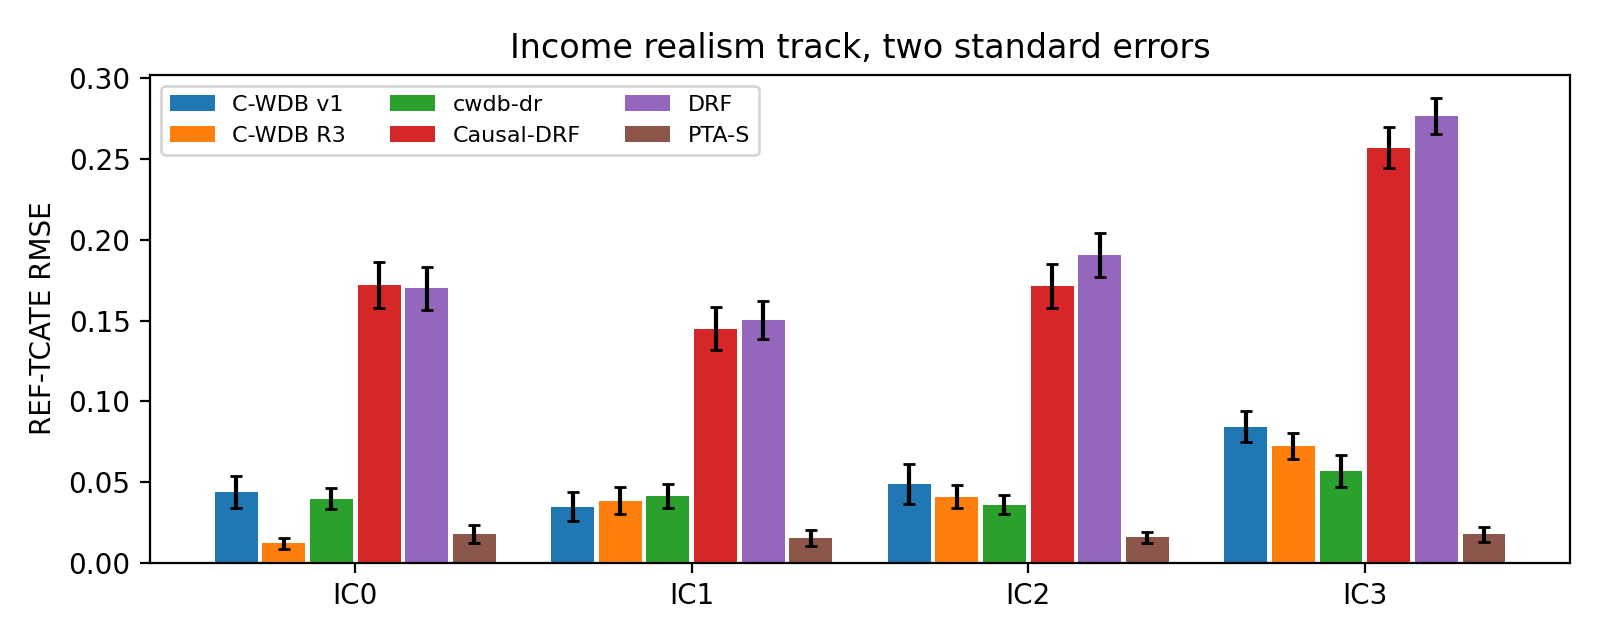
\includegraphics[width=0.9\textwidth]{figures_generated/phase6_income_ref.png}
\caption{Reference TCATE on the income realism track, two standard errors.
The incumbent forests are off scale relative to every C-WDB variant and to
PTA-S on all four regimes, including the placebo.}
\label{fig:p6-income}
\end{figure}

\subsection{Gates, cost, and what this phase supports}
\label{sub:p6-verdict}

Table~\ref{tab:p6-gates} evaluates the six preregistered rules on the merged
record. R1 is PARTIAL, R2 passes fully, R3 fails, R4 and R5 return the
negative and positive descriptive results described above, and R6 records the
reversal. Cost medians are in Table~\ref{tab:p6-cost}: on a loaded machine the
calibration layer runs at roughly thirteen times Causal-DRF, well inside the
inherited cap of sixty, with most of its cost being the cross-fitted booster
it sits on rather than the layer itself, which adds nuisance fits and one set
of fold refits.

Four statements, and no more than four.

First, the doubly-robust calibration layer is the phase's contribution
candidate. It converts the project's worst comparison, the reference-distribution
targets on D5 and the family-wide D0 floor, into parity with the incumbents on
the marginal version and a factor-two improvement over the claimant's own past
on the conditional version; it does this while provably leaving every law-level
property of R3 untouched; it transfers to endogenous-adoption panels where it
is strongest; and it preserves the entire unseen-functional transfer story
because it needs only realised-arm evaluations of whatever functional is named
afterwards. Its price is stated: variance on null and heavily confounded
conditional targets, which argues for reporting it alongside R3 as the
reference-effect estimator rather than as a replacement.

Second, dispersion repair and the smooth weak learner are negative findings
with mechanisms, not tuning failures. Cloud smoothing belongs to D6 and harms
shape functionals elsewhere; smooth base learners memorise the idiosyncratic
component of proper-score gradients unless regularised into averaging, at
which point trees are at least as good. The question "are random forests too
basic" has, for this architecture, a specific answer: the tree's crudeness is
what averages the score.

Third, the functional R-learner is the right new benchmark. It dominates scale
contrasts, is the most null-safe estimator in the project on both mean and
functional targets, and loses where contrasts are near-constant or live purely
inside nonlinear shape, which maps exactly onto where a law-based method is
supposed to be used anyway.

Fourth, the realism audit changes how the applied study should be pitched.
On panels shaped like the intended application, the published incumbent
baselines are the fragile methods, manufacturing large false reference effects
under endogenous adoption even on placebos, while the proposed family holds
and its calibrated version leads. The abstract-suite embarrassment on D5 and
D6 was real but was a representation artefact of outer-law-only contrasts at
ten particles, diagnosed and largely repaired; it is not evidence that the
method loses on realistic problems. If anything the risk runs the other way:
the applied study's headline should be pre-registered around the reference
targets, where the method now has parity-to-superior results and its
competitors have a documented failure mode, and the collaboration with
collaborators on IPUMS CPS state-year extracts is the natural test of whether
the synthetic reversal survives contact with real policy variation.

\subsection{Scope limits}

Ten seeds, sample sizes 500 and 1000, grid resolution K = 25, ten particles
except where stated, and no interval construction anywhere: none of the
variants carries uncertainty guarantees, and the estimand contract still
forbids relabelling posterior quantities. The income track's propensities,
surfaces, and benchmark reference are declared in the preregistration and were
not tuned against any method's performance. Track A speaks only to D0, D2, D5,
D6, D7 and D8; nothing here updates the D1, D3, D4 or D9 record of earlier
phases except through the identity of the underlying R3 law.

% ---- diag
\begin{table}[htbp]
\centering
\caption{Under-dispersion diagnostic: mean bias of the C-WDB-v1 reference-distance expectation against quadrature truth, pooled over five pilot seeds at $n=500$. Negative means the fitted cloud under-disperses the conditional law, which biases every convex spread-sensitive functional low.}
\label{tab:p6-diag}
\small
\begin{tabular}{@{}lrr@{}}
\toprule
Regime & Arm 0 bias & Arm 1 bias \\ 
\midrule
D5 & -0.1494 & -0.0001 \\ 
D6 & -0.3088 & -0.3151 \\ 
D1 & -0.0723 & -0.1020 \\ 
\bottomrule
\end{tabular}
\end{table}


% ---- trackA_reference_effect_rmse
\begin{table}[htbp]
\centering
\caption{REF-ATE-K on the Track A regimes, frozen main coordinates, ten seeds, both sample sizes pooled. Standard errors in parentheses; bold marks the best method.}
\label{tab:p6-tracka-reference_effect_rmse}
\small
\begin{tabular}{@{}lrrrrrrrrrr@{}}
\toprule
Regime & C-WDB v1 & C-WDB R3 & cwdb\_dr & cwdb\_smooth & cwdb\_krr & cwdb\_frl & Causal-DRF & DRF & W-DRF-T & PTA-S \\ 
\midrule
D0 & 0.0419 (0.0017) & 0.0385 (0.0014) & 0.0058 (0.0012) & 0.0382 (0.0014) & 0.0281 (0.0030) & 0.0403 (0.0020) & 0.0129 (0.0024) & 0.0102 (0.0030) & 0.0094 (0.0022) & \textbf{0.0047 (0.0009)} \\ 
D2 & 0.0207 (0.0039) & 0.0096 (0.0026) & 0.0183 (0.0044) & \textbf{0.0090 (0.0023)} & 0.0332 (0.0063) & 0.0097 (0.0024) & 0.0195 (0.0049) & 0.0182 (0.0045) & 0.0193 (0.0052) & 0.0169 (0.0046) \\ 
D5 & 0.0953 (0.0062) & 0.1115 (0.0050) & 0.0232 (0.0044) & 0.0868 (0.0128) & 0.0322 (0.0053) & 0.0451 (0.0079) & 0.0212 (0.0041) & \textbf{0.0189 (0.0040)} & 0.0198 (0.0042) & 0.0195 (0.0038) \\ 
D6 & 0.0479 (0.0088) & 0.0255 (0.0044) & 0.0378 (0.0080) & 0.0268 (0.0041) & 0.0672 (0.0100) & \textbf{0.0139 (0.0031)} & 0.0431 (0.0075) & 0.0414 (0.0072) & 0.0361 (0.0061) & 0.0407 (0.0072) \\ 
D7 & 0.0199 (0.0029) & \textbf{0.0150 (0.0032)} & 0.0180 (0.0038) & 0.0295 (0.0039) & 0.0272 (0.0044) & 0.0364 (0.0051) & 0.0174 (0.0042) & 0.0167 (0.0038) & 0.0170 (0.0040) & 0.0158 (0.0039) \\ 
D8 & 0.0315 (0.0057) & \textbf{0.0238 (0.0027)} & 0.0411 (0.0062) & 0.0246 (0.0027) & 0.0565 (0.0066) & 0.0261 (0.0040) & 0.0491 (0.0079) & 0.0667 (0.0098) & 0.0539 (0.0084) & 0.0412 (0.0056) \\ 
\bottomrule
\end{tabular}
\end{table}


% ---- trackA_reference_tcate_rmse
\begin{table}[htbp]
\centering
\caption{REF-TCATE-K on the Track A regimes, frozen main coordinates, ten seeds, both sample sizes pooled. Standard errors in parentheses; bold marks the best method.}
\label{tab:p6-tracka-reference_tcate_rmse}
\small
\begin{tabular}{@{}lrrrrrrrrrr@{}}
\toprule
Regime & C-WDB v1 & C-WDB R3 & cwdb\_dr & cwdb\_smooth & cwdb\_krr & cwdb\_frl & Causal-DRF & DRF & W-DRF-T & PTA-S \\ 
\midrule
D0 & 0.0575 (0.0018) & 0.0496 (0.0017) & \textbf{0.0155 (0.0017)} & 0.0493 (0.0017) & 0.0696 (0.0053) & 0.0511 (0.0025) & 0.1033 (0.0038) & 0.1113 (0.0075) & 0.0669 (0.0039) & 0.0174 (0.0018) \\ 
D2 & 0.0324 (0.0038) & 0.0184 (0.0029) & 0.0490 (0.0039) & 0.0161 (0.0026) & 0.0703 (0.0057) & \textbf{0.0112 (0.0028)} & 0.0287 (0.0044) & 0.0301 (0.0044) & 0.0361 (0.0051) & 0.0235 (0.0042) \\ 
D5 & 0.1000 (0.0060) & 0.1151 (0.0048) & 0.0549 (0.0062) & 0.0944 (0.0115) & 0.0695 (0.0056) & 0.0589 (0.0071) & 0.0332 (0.0045) & 0.0302 (0.0040) & 0.0358 (0.0047) & \textbf{0.0289 (0.0041)} \\ 
D6 & 0.0765 (0.0084) & 0.0386 (0.0047) & 0.1081 (0.0100) & 0.0400 (0.0047) & 0.1007 (0.0102) & \textbf{0.0215 (0.0036)} & 0.0678 (0.0068) & 0.0632 (0.0064) & 0.0668 (0.0061) & 0.0540 (0.0070) \\ 
D7 & 0.0299 (0.0024) & \textbf{0.0232 (0.0027)} & 0.0449 (0.0038) & 0.0345 (0.0035) & 0.0611 (0.0054) & 0.0440 (0.0043) & 0.0294 (0.0035) & 0.0296 (0.0035) & 0.0336 (0.0039) & 0.0244 (0.0034) \\ 
D8 & 0.0584 (0.0049) & \textbf{0.0444 (0.0035)} & 0.1023 (0.0087) & 0.0450 (0.0034) & 0.2493 (0.0133) & 0.0546 (0.0031) & 0.0695 (0.0067) & 0.0866 (0.0078) & 0.0872 (0.0057) & 0.0624 (0.0038) \\ 
\bottomrule
\end{tabular}
\end{table}


% ---- trackA_paired_ref
\begin{table}[htbp]
\centering
\caption{Seed-paired differences on the reference targets (claimant minus comparator), negative favouring the claimant. An asterisk marks a difference beyond two paired standard errors.}
\label{tab:p6-trackA-paired-ref}
\small
\begin{tabular}{@{}lrrrrrrr@{}}
\toprule
Pair & Target & D0 & D2 & D5 & D6 & D7 & D8 \\ 
\midrule
cwdb\_dr vs cwdb\_r3\_cvridge & effect & -0.0327 (0.0016)$^\ast$ & +0.0087 (0.0043) & -0.0883 (0.0081)$^\ast$ & +0.0122 (0.0106) & +0.0030 (0.0030) & +0.0173 (0.0073) \\ 
cwdb\_dr vs cwdb\_r3\_cvridge & tcate & -0.0341 (0.0024)$^\ast$ & +0.0306 (0.0050) & -0.0602 (0.0080)$^\ast$ & +0.0695 (0.0114) & +0.0218 (0.0043) & +0.0579 (0.0095) \\ 
cwdb\_smooth vs cwdb\_r3\_cvridge & effect & -0.0003 (0.0003) & -0.0006 (0.0005) & -0.0247 (0.0130) & +0.0013 (0.0021) & +0.0145 (0.0031) & +0.0008 (0.0003) \\ 
cwdb\_smooth vs cwdb\_r3\_cvridge & tcate & -0.0003 (0.0003) & -0.0023 (0.0004)$^\ast$ & -0.0207 (0.0114) & +0.0015 (0.0016) & +0.0114 (0.0023) & +0.0006 (0.0003) \\ 
cwdb\_krr vs cwdb\_r3\_cvridge & effect & -0.0103 (0.0036)$^\ast$ & +0.0236 (0.0067) & -0.0793 (0.0091)$^\ast$ & +0.0417 (0.0098) & +0.0122 (0.0049) & +0.0327 (0.0076) \\ 
cwdb\_krr vs cwdb\_r3\_cvridge & tcate & +0.0200 (0.0061) & +0.0519 (0.0061) & -0.0456 (0.0093)$^\ast$ & +0.0621 (0.0103) & +0.0379 (0.0053) & +0.2049 (0.0126) \\ 
cwdb\_frl vs cwdb\_r3\_cvridge & effect & +0.0018 (0.0028) & +0.0001 (0.0029) & -0.0664 (0.0079)$^\ast$ & -0.0117 (0.0069) & +0.0214 (0.0042) & +0.0023 (0.0036) \\ 
cwdb\_frl vs cwdb\_r3\_cvridge & tcate & +0.0015 (0.0035) & -0.0072 (0.0037) & -0.0563 (0.0067)$^\ast$ & -0.0171 (0.0063)$^\ast$ & +0.0208 (0.0033) & +0.0102 (0.0040) \\ 
cwdb\_r3\_cvridge vs causal\_drf & effect & +0.0256 (0.0030) & -0.0099 (0.0050)$^\ast$ & +0.0903 (0.0076) & -0.0176 (0.0100) & -0.0024 (0.0033) & -0.0253 (0.0093)$^\ast$ \\ 
cwdb\_r3\_cvridge vs causal\_drf & tcate & -0.0537 (0.0039)$^\ast$ & -0.0103 (0.0052) & +0.0819 (0.0073) & -0.0292 (0.0089)$^\ast$ & -0.0063 (0.0030)$^\ast$ & -0.0251 (0.0071)$^\ast$ \\ 
\bottomrule
\end{tabular}
\end{table}


% ---- trackA_kernel_law_error
\begin{table}[htbp]
\centering
\caption{Primary law metric across the Track A regimes (ten seeds, sample sizes pooled).}
\label{tab:p6-trackA-kernel_law_error}
\small
\begin{tabular}{@{}lrrrrrrrrrr@{}}
\toprule
Regime & C-WDB v1 & C-WDB R3 & cwdb\_dr & cwdb\_smooth & cwdb\_krr & cwdb\_frl & Causal-DRF & DRF & W-DRF-T & PTA-S \\ 
\midrule
D0 & \textbf{0.0266 (0.0013)} & 0.0287 (0.0016) & 0.0287 (0.0016) & 0.0288 (0.0016) & 0.0771 (0.0032) & \emph{n/a} & 0.1209 (0.0049) & 0.1422 (0.0061) & 0.1008 (0.0041) & \emph{n/a} \\ 
D2 & 0.0129 (0.0006) & \textbf{0.0122 (0.0006)} & \textbf{0.0122 (0.0006)} & 0.0128 (0.0007) & 0.0285 (0.0007) & \emph{n/a} & 0.0188 (0.0008) & 0.0163 (0.0006) & 0.0125 (0.0004) & \emph{n/a} \\ 
D5 & 0.0244 (0.0010) & \textbf{0.0236 (0.0007)} & \textbf{0.0236 (0.0007)} & 0.0257 (0.0008) & 0.0470 (0.0010) & \emph{n/a} & 0.0444 (0.0019) & 0.0492 (0.0016) & 0.0368 (0.0013) & \emph{n/a} \\ 
D6 & 0.0279 (0.0022) & 0.0254 (0.0019) & 0.0254 (0.0019) & 0.0182 (0.0014) & 0.0376 (0.0027) & \emph{n/a} & 0.0078 (0.0005) & 0.0083 (0.0007) & \textbf{0.0065 (0.0003)} & \emph{n/a} \\ 
D7 & 0.0129 (0.0006) & \textbf{0.0117 (0.0006)} & \textbf{0.0117 (0.0006)} & 0.0123 (0.0006) & 0.0282 (0.0007) & \emph{n/a} & 0.0159 (0.0007) & 0.0170 (0.0007) & 0.0131 (0.0004) & \emph{n/a} \\ 
D8 & 0.0181 (0.0007) & \textbf{0.0155 (0.0007)} & \textbf{0.0155 (0.0007)} & 0.0161 (0.0007) & 0.0657 (0.0014) & \emph{n/a} & 0.0498 (0.0021) & 0.0483 (0.0017) & 0.0385 (0.0013) & \emph{n/a} \\ 
\bottomrule
\end{tabular}
\end{table}


% ---- trackA_mean_quantile_rmse
\begin{table}[htbp]
\centering
\caption{Grid causal mean contrast across the Track A regimes (ten seeds, sample sizes pooled).}
\label{tab:p6-trackA-mean_quantile_rmse}
\small
\begin{tabular}{@{}lrrrrrrrrrr@{}}
\toprule
Regime & C-WDB v1 & C-WDB R3 & cwdb\_dr & cwdb\_smooth & cwdb\_krr & cwdb\_frl & Causal-DRF & DRF & W-DRF-T & PTA-S \\ 
\midrule
D0 & 0.1106 (0.0030) & 0.0943 (0.0021) & 0.0943 (0.0021) & 0.0943 (0.0021) & 0.1662 (0.0058) & 0.0967 (0.0036) & 0.1637 (0.0057) & 0.1920 (0.0060) & 0.1423 (0.0044) & \textbf{0.0544 (0.0018)} \\ 
D2 & 0.1462 (0.0053) & 0.0595 (0.0113) & 0.0595 (0.0113) & 0.0590 (0.0112) & 0.3526 (0.0080) & \textbf{0.0169 (0.0020)} & 0.0952 (0.0068) & 0.0743 (0.0063) & 0.0948 (0.0044) & 0.0551 (0.0038) \\ 
D5 & 0.1759 (0.0050) & 0.1728 (0.0190) & 0.1728 (0.0190) & 0.1712 (0.0187) & 0.3699 (0.0118) & \textbf{0.0269 (0.0038)} & 0.0907 (0.0057) & 0.1028 (0.0068) & 0.1103 (0.0046) & 0.0499 (0.0043) \\ 
D6 & 0.3042 (0.0163) & 0.2563 (0.0145) & 0.2563 (0.0145) & 0.2563 (0.0145) & 0.6667 (0.0305) & 0.3577 (0.0094) & 0.2723 (0.0159) & \textbf{0.2273 (0.0155)} & 0.2379 (0.0095) & 0.2409 (0.0120) \\ 
D7 & 0.1456 (0.0049) & 0.0661 (0.0033) & 0.0661 (0.0033) & 0.0688 (0.0031) & 0.3494 (0.0072) & 0.1083 (0.0040) & 0.0871 (0.0064) & 0.0787 (0.0065) & 0.0966 (0.0044) & \textbf{0.0637 (0.0034)} \\ 
D8 & 0.1793 (0.0058) & 0.0739 (0.0033) & 0.0739 (0.0033) & \textbf{0.0738 (0.0033)} & 0.5831 (0.0113) & 0.0859 (0.0027) & 0.2513 (0.0134) & 0.1843 (0.0082) & 0.2008 (0.0058) & 0.0984 (0.0046) \\ 
\bottomrule
\end{tabular}
\end{table}


% ---- trackA_mode_coverage
\begin{table}[htbp]
\centering
\caption{Mode coverage across the Track A regimes (ten seeds, sample sizes pooled).}
\label{tab:p6-trackA-mode_coverage}
\small
\begin{tabular}{@{}lrrrrrrrrrr@{}}
\toprule
Regime & C-WDB v1 & C-WDB R3 & cwdb\_dr & cwdb\_smooth & cwdb\_krr & cwdb\_frl & Causal-DRF & DRF & W-DRF-T & PTA-S \\ 
\midrule
D0 & \textbf{1.0000 (0.0000)} & \textbf{1.0000 (0.0000)} & \textbf{1.0000 (0.0000)} & \textbf{1.0000 (0.0000)} & \textbf{1.0000 (0.0000)} & \emph{n/a} & \textbf{1.0000 (0.0000)} & \textbf{1.0000 (0.0000)} & \textbf{1.0000 (0.0000)} & \emph{n/a} \\ 
D2 & \textbf{1.0000 (0.0000)} & \textbf{1.0000 (0.0000)} & \textbf{1.0000 (0.0000)} & \textbf{1.0000 (0.0000)} & 0.9999 (0.0001) & \emph{n/a} & \textbf{1.0000 (0.0000)} & \textbf{1.0000 (0.0000)} & \textbf{1.0000 (0.0000)} & \emph{n/a} \\ 
D5 & \textbf{1.0000 (0.0000)} & \textbf{1.0000 (0.0000)} & \textbf{1.0000 (0.0000)} & \textbf{1.0000 (0.0000)} & 0.9992 (0.0003) & \emph{n/a} & \textbf{1.0000 (0.0000)} & \textbf{1.0000 (0.0000)} & \textbf{1.0000 (0.0000)} & \emph{n/a} \\ 
D6 & 0.9879 (0.0032) & 0.9937 (0.0015) & 0.9937 (0.0015) & 0.9944 (0.0014) & 0.9687 (0.0052) & \emph{n/a} & \textbf{1.0000 (0.0000)} & \textbf{1.0000 (0.0000)} & \textbf{1.0000 (0.0000)} & \emph{n/a} \\ 
D7 & \textbf{1.0000 (0.0000)} & \textbf{1.0000 (0.0000)} & \textbf{1.0000 (0.0000)} & \textbf{1.0000 (0.0000)} & 0.9998 (0.0002) & \emph{n/a} & \textbf{1.0000 (0.0000)} & \textbf{1.0000 (0.0000)} & \textbf{1.0000 (0.0000)} & \emph{n/a} \\ 
D8 & \textbf{1.0000 (0.0000)} & \textbf{1.0000 (0.0000)} & \textbf{1.0000 (0.0000)} & \textbf{1.0000 (0.0000)} & 0.9829 (0.0026) & \emph{n/a} & \textbf{1.0000 (0.0000)} & \textbf{1.0000 (0.0000)} & \textbf{1.0000 (0.0000)} & \emph{n/a} \\ 
\bottomrule
\end{tabular}
\end{table}


% ---- tcate_trackA
\begin{table}[htbp]
\centering
\caption{TCATE error by functional and regime. Skewness and the upper-tail mean are excluded from every training manifest; a method can only produce them from a full law, by orthogonalisation, or not at all.}
\label{tab:p6-trackA-tcate}
\small
\begin{tabular}{@{}lrrrrrrrrrrr@{}}
\toprule
Functional & Regime & C-WDB v1 & C-WDB R3 & cwdb\_dr & cwdb\_smooth & cwdb\_krr & cwdb\_frl & Causal-DRF & DRF & W-DRF-T & PTA-S \\ 
\midrule
grid\_sd & D0 & 0.0196 (0.0015) & 0.0101 (0.0008) & 0.0166 (0.0016) & 0.0101 (0.0008) & 0.0169 (0.0015) & 0.0058 (0.0006) & 0.0171 (0.0014) & 0.0168 (0.0015) & 0.0133 (0.0014) & \textbf{0.0012 (0.0001)} \\ 
grid\_sd & D2 & 0.0291 (0.0030) & 0.0173 (0.0019) & 0.0381 (0.0035) & 0.0168 (0.0018) & 0.0465 (0.0030) & \textbf{0.0052 (0.0011)} & 0.0180 (0.0022) & 0.0182 (0.0020) & 0.0207 (0.0021) & 0.0149 (0.0017) \\ 
grid\_sd & D5 & 0.0481 (0.0046) & 0.0469 (0.0045) & 0.0573 (0.0064) & 0.0461 (0.0044) & 0.0711 (0.0064) & \textbf{0.0085 (0.0017)} & 0.0336 (0.0034) & 0.0287 (0.0038) & 0.0308 (0.0043) & 0.0209 (0.0040) \\ 
grid\_sd & D6 & 0.0233 (0.0023) & 0.0132 (0.0014) & 0.0273 (0.0028) & 0.0132 (0.0014) & 0.0327 (0.0021) & \textbf{0.0053 (0.0011)} & 0.0162 (0.0018) & 0.0140 (0.0018) & 0.0160 (0.0019) & 0.0115 (0.0014) \\ 
grid\_sd & D7 & 0.0303 (0.0027) & 0.0182 (0.0020) & 0.0359 (0.0035) & 0.0177 (0.0019) & 0.0454 (0.0029) & \textbf{0.0151 (0.0008)} & 0.0198 (0.0023) & 0.0182 (0.0020) & 0.0209 (0.0023) & 0.0155 (0.0015) \\ 
grid\_sd & D8 & 0.0346 (0.0032) & 0.0173 (0.0022) & 0.0605 (0.0070) & 0.0169 (0.0021) & 0.0520 (0.0043) & \textbf{0.0079 (0.0013)} & 0.0267 (0.0020) & 0.0238 (0.0021) & 0.0257 (0.0019) & 0.0201 (0.0020) \\ 
grid\_skewness & D0 & 0.0016 (0.0002) & 0.0120 (0.0023) & 0.0012 (0.0001) & 0.0120 (0.0023) & 0.0040 (0.0006) & \textbf{0.0000 (0.0000)} & \textbf{0.0000 (0.0000)} & \textbf{0.0000 (0.0000)} & \textbf{0.0000 (0.0000)} & \emph{n/a} \\ 
grid\_skewness & D2 & 0.0000 (0.0000) & 0.0000 (0.0000) & 0.0000 (0.0000) & 0.0002 (0.0000) & 0.0019 (0.0005) & \textbf{0.0000 (0.0000)} & \textbf{0.0000 (0.0000)} & \textbf{0.0000 (0.0000)} & \textbf{0.0000 (0.0000)} & \emph{n/a} \\ 
grid\_skewness & D5 & 0.0122 (0.0023) & 0.0035 (0.0012) & 0.0013 (0.0004) & 0.0035 (0.0011) & 0.0045 (0.0009) & \textbf{0.0000 (0.0000)} & \textbf{0.0000 (0.0000)} & \textbf{0.0000 (0.0000)} & \textbf{0.0000 (0.0000)} & \emph{n/a} \\ 
grid\_skewness & D6 & \textbf{0.0000 (0.0000)} & \textbf{0.0000 (0.0000)} & \textbf{0.0000 (0.0000)} & 0.0000 (0.0000) & 0.0028 (0.0007) & \textbf{0.0000 (0.0000)} & \textbf{0.0000 (0.0000)} & \textbf{0.0000 (0.0000)} & \textbf{0.0000 (0.0000)} & \emph{n/a} \\ 
grid\_skewness & D7 & 0.0152 (0.0014) & 0.0860 (0.0066) & 0.0199 (0.0026) & 0.1550 (0.0078) & \textbf{0.0119 (0.0011)} & 0.1271 (0.0048) & 0.0514 (0.0032) & 0.0580 (0.0025) & 0.0466 (0.0016) & \emph{n/a} \\ 
grid\_skewness & D8 & \textbf{0.0000 (0.0000)} & \textbf{0.0000 (0.0000)} & 0.0000 (0.0000) & 0.0001 (0.0000) & 0.0094 (0.0014) & \textbf{0.0000 (0.0000)} & \textbf{0.0000 (0.0000)} & \textbf{0.0000 (0.0000)} & \textbf{0.0000 (0.0000)} & \emph{n/a} \\ 
grid\_upper\_tail\_mean & D0 & 0.0878 (0.0034) & 0.0551 (0.0018) & \textbf{0.0226 (0.0021)} & 0.0551 (0.0018) & 0.0976 (0.0064) & 0.0526 (0.0028) & 0.1223 (0.0062) & 0.1129 (0.0086) & 0.0682 (0.0046) & \emph{n/a} \\ 
grid\_upper\_tail\_mean & D2 & 0.0606 (0.0050) & 0.0311 (0.0044) & 0.0669 (0.0065) & 0.0310 (0.0043) & 0.1073 (0.0088) & \textbf{0.0071 (0.0011)} & 0.0784 (0.0087) & 0.0567 (0.0083) & 0.0565 (0.0065) & \emph{n/a} \\ 
grid\_upper\_tail\_mean & D5 & 0.0663 (0.0067) & 0.0607 (0.0062) & 0.0730 (0.0075) & 0.0605 (0.0062) & 0.1183 (0.0084) & \textbf{0.0117 (0.0025)} & 0.0663 (0.0070) & 0.0764 (0.0090) & 0.0658 (0.0067) & \emph{n/a} \\ 
grid\_upper\_tail\_mean & D6 & 0.2211 (0.0189) & 0.2310 (0.0161) & 0.2235 (0.0235) & 0.2310 (0.0161) & 0.2664 (0.0260) & 0.3132 (0.0151) & 0.2196 (0.0193) & 0.2017 (0.0170) & \textbf{0.1813 (0.0127)} & \emph{n/a} \\ 
grid\_upper\_tail\_mean & D7 & 0.0534 (0.0060) & \textbf{0.0330 (0.0037)} & 0.0702 (0.0059) & 0.0332 (0.0038) & 0.1026 (0.0071) & 0.0412 (0.0035) & 0.0643 (0.0082) & 0.0572 (0.0086) & 0.0569 (0.0064) & \emph{n/a} \\ 
grid\_upper\_tail\_mean & D8 & 0.0918 (0.0091) & 0.0596 (0.0038) & 0.1283 (0.0095) & \textbf{0.0595 (0.0038)} & 0.2961 (0.0129) & 0.0660 (0.0040) & 0.2207 (0.0165) & 0.1361 (0.0121) & 0.1104 (0.0082) & \emph{n/a} \\ 
\bottomrule
\end{tabular}
\end{table}


% ---- tcate_incomeB
\begin{table}[htbp]
\centering
\caption{TCATE error by functional and regime. Skewness and the upper-tail mean are excluded from every training manifest; a method can only produce them from a full law, by orthogonalisation, or not at all.}
\label{tab:p6-incomeB-tcate}
\small
\begin{tabular}{@{}lrrrrrrr@{}}
\toprule
Functional & Regime & C-WDB v1 & C-WDB R3 & cwdb\_dr & Causal-DRF & DRF & PTA-S \\ 
\midrule
grid\_sd & IC0 & 0.0150 (0.0016) & 0.0104 (0.0016) & 0.0271 (0.0020) & 0.0093 (0.0015) & \textbf{0.0088 (0.0015)} & 0.0095 (0.0014) \\ 
grid\_sd & IC1 & 0.0155 (0.0016) & 0.0143 (0.0019) & 0.0276 (0.0027) & 0.0084 (0.0013) & \textbf{0.0079 (0.0013)} & 0.0096 (0.0014) \\ 
grid\_sd & IC2 & 0.0164 (0.0015) & 0.0180 (0.0022) & 0.0279 (0.0022) & 0.0085 (0.0014) & \textbf{0.0073 (0.0012)} & 0.0086 (0.0012) \\ 
grid\_sd & IC3 & 0.0160 (0.0018) & 0.0151 (0.0017) & 0.0388 (0.0036) & 0.0087 (0.0012) & \textbf{0.0081 (0.0012)} & 0.0085 (0.0015) \\ 
grid\_skewness & IC0 & 0.0164 (0.0015) & \textbf{0.0079 (0.0013)} & 0.0129 (0.0015) & 0.0750 (0.0026) & 0.0713 (0.0028) & \emph{n/a} \\ 
grid\_skewness & IC1 & \textbf{0.0164 (0.0018)} & 0.0348 (0.0058) & 0.0165 (0.0015) & 0.0519 (0.0018) & 0.0530 (0.0017) & \emph{n/a} \\ 
grid\_skewness & IC2 & 0.0200 (0.0019) & 0.0290 (0.0035) & \textbf{0.0129 (0.0013)} & 0.0848 (0.0030) & 0.0988 (0.0024) & \emph{n/a} \\ 
grid\_skewness & IC3 & \textbf{0.0286 (0.0022)} & 0.0443 (0.0053) & 0.0312 (0.0032) & 0.0852 (0.0028) & 0.0982 (0.0025) & \emph{n/a} \\ 
grid\_upper\_tail\_mean & IC0 & 0.0631 (0.0058) & \textbf{0.0176 (0.0020)} & 0.0443 (0.0041) & 0.2114 (0.0083) & 0.2083 (0.0077) & \emph{n/a} \\ 
grid\_upper\_tail\_mean & IC1 & 0.0535 (0.0068) & 0.0552 (0.0043) & \textbf{0.0528 (0.0042)} & 0.1839 (0.0081) & 0.1912 (0.0068) & \emph{n/a} \\ 
grid\_upper\_tail\_mean & IC2 & 0.0668 (0.0068) & 0.0436 (0.0036) & \textbf{0.0431 (0.0043)} & 0.2192 (0.0079) & 0.2405 (0.0071) & \emph{n/a} \\ 
grid\_upper\_tail\_mean & IC3 & 0.1112 (0.0071) & 0.0904 (0.0063) & \textbf{0.0618 (0.0045)} & 0.3325 (0.0073) & 0.3587 (0.0063) & \emph{n/a} \\ 
\bottomrule
\end{tabular}
\end{table}


% ---- income_mean_quantile_rmse
\begin{table}[htbp]
\centering
\caption{Grid causal mean contrast on the income realism track (six methods, ten seeds, sample sizes pooled).}
\label{tab:p6-income-mean_quantile_rmse}
\small
\begin{tabular}{@{}lrrrrrr@{}}
\toprule
Regime & C-WDB v1 & C-WDB R3 & cwdb\_dr & Causal-DRF & DRF & PTA-S \\ 
\midrule
IC0 & 0.1251 (0.0038) & 0.0498 (0.0075) & \textbf{0.0430 (0.0077)} & 0.2135 (0.0079) & 0.2151 (0.0071) & 0.0433 (0.0021) \\ 
IC1 & 0.1225 (0.0033) & 0.1276 (0.0072) & 0.1166 (0.0085) & 0.1935 (0.0079) & 0.2035 (0.0066) & \textbf{0.0606 (0.0021)} \\ 
IC2 & 0.1281 (0.0042) & 0.1029 (0.0088) & 0.0843 (0.0089) & 0.2152 (0.0075) & 0.2397 (0.0071) & \textbf{0.0433 (0.0025)} \\ 
IC3 & 0.1585 (0.0045) & 0.1539 (0.0068) & 0.1259 (0.0055) & 0.3311 (0.0071) & 0.3584 (0.0061) & \textbf{0.0750 (0.0027)} \\ 
\bottomrule
\end{tabular}
\end{table}


% ---- income_reference_effect_rmse
\begin{table}[htbp]
\centering
\caption{Reference marginal effect on the income realism track (six methods, ten seeds, sample sizes pooled).}
\label{tab:p6-income-reference_effect_rmse}
\small
\begin{tabular}{@{}lrrrrrr@{}}
\toprule
Regime & C-WDB v1 & C-WDB R3 & cwdb\_dr & Causal-DRF & DRF & PTA-S \\ 
\midrule
IC0 & 0.0417 (0.0050) & \textbf{0.0085 (0.0019)} & 0.0194 (0.0026) & 0.1719 (0.0072) & 0.1700 (0.0067) & 0.0147 (0.0027) \\ 
IC1 & 0.0319 (0.0047) & 0.0352 (0.0046) & 0.0218 (0.0035) & 0.1446 (0.0067) & 0.1502 (0.0059) & \textbf{0.0128 (0.0027)} \\ 
IC2 & 0.0463 (0.0064) & 0.0386 (0.0040) & 0.0164 (0.0021) & 0.1713 (0.0069) & 0.1905 (0.0067) & \textbf{0.0132 (0.0017)} \\ 
IC3 & 0.0832 (0.0049) & 0.0703 (0.0042) & 0.0223 (0.0039) & 0.2568 (0.0065) & 0.2767 (0.0056) & \textbf{0.0161 (0.0024)} \\ 
\bottomrule
\end{tabular}
\end{table}


% ---- income_reference_tcate_rmse
\begin{table}[htbp]
\centering
\caption{Reference TCATE on the income realism track (six methods, ten seeds, sample sizes pooled).}
\label{tab:p6-income-reference_tcate_rmse}
\small
\begin{tabular}{@{}lrrrrrr@{}}
\toprule
Regime & C-WDB v1 & C-WDB R3 & cwdb\_dr & Causal-DRF & DRF & PTA-S \\ 
\midrule
IC0 & 0.0435 (0.0049) & \textbf{0.0118 (0.0017)} & 0.0397 (0.0033) & 0.1721 (0.0072) & 0.1701 (0.0066) & 0.0176 (0.0028) \\ 
IC1 & 0.0346 (0.0044) & 0.0384 (0.0041) & 0.0411 (0.0038) & 0.1449 (0.0066) & 0.1503 (0.0059) & \textbf{0.0153 (0.0024)} \\ 
IC2 & 0.0486 (0.0062) & 0.0409 (0.0036) & 0.0358 (0.0029) & 0.1715 (0.0069) & 0.1906 (0.0067) & \textbf{0.0156 (0.0016)} \\ 
IC3 & 0.0842 (0.0049) & 0.0720 (0.0040) & 0.0565 (0.0049) & 0.2571 (0.0064) & 0.2769 (0.0055) & \textbf{0.0174 (0.0022)} \\ 
\bottomrule
\end{tabular}
\end{table}


% ---- income_kernel_law_error
\begin{table}[htbp]
\centering
\caption{Primary law metric on the income realism track (six methods, ten seeds, sample sizes pooled).}
\label{tab:p6-income-kernel_law_error}
\small
\begin{tabular}{@{}lrrrrrr@{}}
\toprule
Regime & C-WDB v1 & C-WDB R3 & cwdb\_dr & Causal-DRF & DRF & PTA-S \\ 
\midrule
IC0 & 0.0191 (0.0008) & \textbf{0.0176 (0.0006)} & 0.0179 (0.0007) & 0.0559 (0.0023) & 0.0773 (0.0032) & \emph{n/a} \\ 
IC1 & \textbf{0.0190 (0.0006)} & 0.0198 (0.0008) & 0.0205 (0.0009) & 0.0541 (0.0023) & 0.0706 (0.0028) & \emph{n/a} \\ 
IC2 & 0.0204 (0.0007) & 0.0201 (0.0009) & \textbf{0.0194 (0.0008)} & 0.0586 (0.0024) & 0.0851 (0.0031) & \emph{n/a} \\ 
IC3 & 0.0223 (0.0010) & 0.0233 (0.0011) & \textbf{0.0216 (0.0009)} & 0.0689 (0.0022) & 0.0866 (0.0026) & \emph{n/a} \\ 
\bottomrule
\end{tabular}
\end{table}


% ---- income_paired
\begin{table}[htbp]
\centering
\caption{Seed-paired difference R3 minus Causal-DRF on the income track, negative favouring R3; asterisk marks significance at two standard errors. This is the realism audit's central comparison.}
\label{tab:p6-income-paired}
\small
\begin{tabular}{@{}lrrrr@{}}
\toprule
Metric & IC0 & IC1 & IC2 & IC3 \\ 
\midrule
kernel\_law\_error & -0.0382 (0.0020)$^\ast$ & -0.0342 (0.0018)$^\ast$ & -0.0385 (0.0019)$^\ast$ & -0.0457 (0.0017)$^\ast$ \\ 
mean\_quantile\_rmse & -0.1637 (0.0120)$^\ast$ & -0.0659 (0.0104)$^\ast$ & -0.1123 (0.0093)$^\ast$ & -0.1771 (0.0099)$^\ast$ \\ 
reference\_effect\_rmse & -0.1634 (0.0071)$^\ast$ & -0.1095 (0.0059)$^\ast$ & -0.1327 (0.0069)$^\ast$ & -0.1865 (0.0059)$^\ast$ \\ 
reference\_tcate\_rmse & -0.1603 (0.0069)$^\ast$ & -0.1066 (0.0054)$^\ast$ & -0.1306 (0.0067)$^\ast$ & -0.1850 (0.0058)$^\ast$ \\ 
\bottomrule
\end{tabular}
\end{table}


% ---- diag_track
\begin{table}[htbp]
\centering
\caption{Variant diagnostics on Track A: the shrinkage each cross-fitted selection chose, the smoothing strength, and the accepted boosting steps. Values are cell means over regimes' ten seeds and both sample sizes.}
\label{tab:p6-diag-track}
\small
\begin{tabular}{@{}lrrrrrr@{}}
\toprule
Diagnostic & D0 & D2 & D5 & D6 & D7 & D8 \\ 
\midrule
cwdb\_dr selected shrinkage & 0.00 & 247.50 & 20.00 & 140.00 & 185.00 & 410.00 \\ 
cwdb\_smooth transform code/value & 1.01 & 0.09 & 0.63 & 1.24 & 0.09 & 0.08 \\ 
cwdb\_krr accepted steps & 100.00 & 98.67 & 94.22 & 91.90 & 100.00 & 100.00 \\ 
cwdb\_frl selected shrinkage & 8.33 & 472.17 & 417.08 & 307.75 & 197.75 & 252.50 \\ 
\bottomrule
\end{tabular}
\end{table}


% ---- cost
\begin{table}[htbp]
\centering
\caption{Runtime medians over the Phase 6 cells. Every number is contaminated by machine load to some degree; the ordering is reliable, the levels are upper bounds.}
\label{tab:p6-cost}
\small
\begin{tabular}{@{}lrrr@{}}
\toprule
Track & Method & Median seconds & Cells \\ 
\midrule
main & C-WDB v1 & 17.2 & 120 \\ 
main & C-WDB R3 & 84.4 & 120 \\ 
main & cwdb\_dr & 197.1 & 120 \\ 
main & cwdb\_smooth & 173.3 & 120 \\ 
main & cwdb\_krr & 15.8 & 120 \\ 
main & cwdb\_frl & 4.1 & 120 \\ 
main & Causal-DRF & 14.7 & 120 \\ 
main & DRF & 11.9 & 120 \\ 
main & W-DRF-T & 1.8 & 120 \\ 
main & PTA-S & 35.7 & 120 \\ 
income & C-WDB v1 & 33.1 & 80 \\ 
income & C-WDB R3 & 140.8 & 80 \\ 
income & cwdb\_dr & 209.2 & 80 \\ 
income & Causal-DRF & 37.8 & 80 \\ 
income & DRF & 39.7 & 80 \\ 
income & PTA-S & 88.0 & 80 \\ 
\bottomrule
\end{tabular}
\end{table}


% ---- gates
\begin{table}[htbp]
\centering
\caption{The preregistered Phase 6 decision rules, evaluated on the merged track. Descriptive rules report direction, not pass or fail.}
\label{tab:p6-gates}
\small
\begin{tabular}{@{}lrr@{}}
\toprule
Rule & Statement & Result \\ 
\midrule
R1\_reference\_repair & DR repairs D5 references without losing D2/D8 & PARTIAL: D5 ATE diff -0.0883 (0.0081), D5 TCATE diff -0.0602 (0.0080); significant losses: D2/effect +0.0087, D2/tcate +0.0306, D8/effect +0.0173, D8/tcate +0.0579 \\ 
R2\_D0 & cwdb\_dr mean\_quantile $\leq$ 0.15 on D0 & PASS (0.0943) \\ 
R2\_D2 & cwdb\_dr mean\_quantile $\leq$ 0.15 on D2 & PASS (0.0595) \\ 
R2\_null\_ratio & D2 false-effect ratio $\leq$ 1.25 vs best baseline & PASS (ratio 1.08) \\ 
R3\_smoothing & smooth improves law metric in >=3/6 regimes, no collapse & FAIL (1/6 significant wins; D6 coverage 0.9944; D0:+0.0001 D2:+0.0006 D5:+0.0021 D6:-0.0072 D7:+0.0006 D8:+0.0007) \\ 
R4\_krr\_probe & descriptive: KRR weak learner vs tree weak learner & negative: loses law metric in 0/6 regimes \\ 
R5\_frl & descriptive: functional R-learner vs R3 on null reference TCATE & FRL wins D2 REF-TCATE by 0.0072 (0.0037) \\ 
R6\_realism & does the R3-vs-CausalDRF ordering reproduce on income? & REVERSED: see income tables; forests lose every law and reference comparison there \\ 
\bottomrule
\end{tabular}
\end{table}

